\documentclass[9pt,twocolumn,twoside]{pnas-new}
% Use the lineno option to display guide line numbers if required.
% Note that the use of elements such as single-column equations
% may affect the guide line number alignment.
\templatetype{pnasresearcharticle} % Choose template
% {pnasresearcharticle} = Template for a two-column research article
% {pnasmathematics} = Template for a one-column mathematics article
% {pnasinvited} = Template for a PNAS invited submission
%\usepackage{graphicx}

\usepackage{amsmath,amsfonts,amssymb}
\usepackage{fullpage}
\usepackage{color}
\usepackage{bm}
\newcommand{\rr}[1]{{\rm #1}}



% \usepackage[english]{babel}
% \usepackage[latin1]{inputenc}
% \usepackage[T1]{fontenc}
% \usepackage{color}
% \usepackage{float}
% \usepackage{verbatim}
% \usepackage{graphicx}
% \usepackage{bm}
% \usepackage{mathtools}
% \usepackage{stmaryrd}
% \usepackage{anyfontsize}
% \usepackage{fullpage}
% \usepackage{color}


\graphicspath{{../Enigma/figures/}}



% \title{Quantization of ecological interactions yields insights into ecosystem assembly and dynamics}
\title{Diverse interactions and ecosystem engineering stabilize assembly of ecological networks}

% Use letters for affiliations, numbers to show equal authorship (if applicable) and to indicate the corresponding author
\author[a,b]{Justin D. Yeakel}
% \author[a,b]{Hattie}
\author[c]{Mathias Pires}
\author[c]{Marcus A. M. de Aguiar}
\author[d]{James O'Donnell}
\author[e]{Paulo R. Guimar\~aes Jr.}
\author[f]{Dominique Gravel}
\author[g]{Thilo Gross}


\affil[a]{School of Natural Sciences, University of California Merced, Merced, CA 95343, USA}
\affil[b]{Santa Fe Institute}
\affil[c]{Universidade Estadual de Campinas}
\affil[d]{University of Washington}
\affil[e]{Universidade de S\~ao Paulo}
\affil[f]{Universit\`e de Sherbrooke}
\affil[g]{University of California Davis, Davis CA}

% Please give the surname of the lead author for the running footer
\leadauthor{Yeakel}

% Please add here a significance statement to explain the relevance of your work
\significancestatement{
Here
%Authors must submit a 120-word maximum statement about the significance of their research paper written at a level understandable to an undergraduate educated scientist outside their field of speciality. The primary goal of the Significance Statement is to explain the relevance of the work in broad context to a broad readership. The Significance Statement appears in the paper itself and is required for all research papers.
}

% Please include corresponding author, author contribution and author declaration information
\authorcontributions{Please provide details of author contributions here.}
\authordeclaration{Please declare any conflict of interest here.}
\correspondingauthor{\textsuperscript{2}To whom correspondence should be addressed. E-mail: jyeakel@ucmerced.edu}

% Keywords are not mandatory, but authors are strongly encouraged to provide them. If provided, please include two to five keywords, separated by the pipe symbol, e.g:
\keywords{Ecosystem assembly $|$ Ecological networks $|$ Colonization $|$ Extinction $|$ Ecosystem engineering}
\begin{abstract}
In this paper we investigate the effects of heterogeneity in food available on the survival times of foraging individuals, using a simple model to incorporate the basic elements of time-stationary foraging process.
\end{abstract}
\dates{This manuscript was compiled on \today}
\doi{\url{www.pnas.org/cgi/doi/10.1073/pnas.XXXXXXXXXX}}



\begin{document}
% Optional adjustment to line up main text (after abstract) of first page with line numbers, when using both lineno and twocolumn options.
% You should only change this length when you've finalised the article contents.
\verticaladjustment{-2pt}

\maketitle
\thispagestyle{firststyle}
\ifthenelse{\boolean{shortarticle}}{\ifthenelse{\boolean{singlecolumn}}{\abscontentformatted}{\abscontent}}{}


%structure is the result of dynamics
Simplifying the abundant complexities and eccentricities of nature is necessary to unravel its secrets.
The layers of natural history giving rise to an ecological community can be distilled -- among many possible forms -- into a network, where nodes represent species and links represent interactions between them.
% to the set of species and the interactions binding those species, and their populations, together.
% An ecological network, where nodes represent species and links represent interactions between species, is
This minimalist perspective provides insight into community structure, and consequently, the dynamics of populations and system stability \cite{May1972}.
Community structure can directly impact the ability of the system to absorb external perturbations \cite{Yeakel2014,Novak2016}, the existence and ubiquity of tipping points that can cause sudden long-term changes in species' populations \cite{Lade2011,Boettiger2012}, and promote or inhibit extinction cascades \cite{Stouffer2011}.
Importantly, community structure is the result of a dynamical process that takes place over time, where species are added to or removed from the community in succession \cite{Weiher2001}.
This process is generally referred to as community assembly (Diamond,Brown,Loreau,Book), and though it is an engine for much that we observe in nature, is not well understood.

%multiple interaction types
Ecological networks are generally constructed and analyzed with respect to a single type of interaction.
For example, beneficial relationships between species form the foundation of mutualistic networks, whereas antagonistic interactions form the foundation of trophic networks, or food webs. %- which are often trophic in one direction and a reproductive service in the other -
More recently, there has been a growing interest in understanding community structure by taking into account diverse interaction types, where multiple unique interactions are included, sometimes in a multi-layer network \cite{Kefi2016,Pilosof2017}.
Interactions between two species are inherently compound in nature, such that both species in an interaction experiences different effects.
For example, mutualistic interactions generally involve a flow of biomass in one direction and a reproductive service in the other; in a trophic interaction there is a flow of biomass from the prey to the predator but not the other way around.
While this asymmetry is generally not encoded in ecological network structure, it is central to the emergent dynamics \cite{Gross2009,Allesina2012}.


%Ecosystem engineering
Diverse interactions occur directly between species, and indirectly through the effects species have on their environment \cite{Jones1994,Olff2009,OdlingSmee2013}.
If these environmental effects have timescales longer than that of the instigating species, they are dubbed ecosystem engineers \cite{Hastings2007}.
Photosynthetic primary producers have engineerd the stoichiometry of the planet, the emergence of multicellular cyanobacteria altering the atmosphere during the Great Oxidation Event \cite{Schirrmeister2013}, to rRNA and protein biogenesis driving the ratio of nitrogen to phosphorous (the Redfield Ratio) to ca. 16:1 in the ocean \cite{Loladze2011}.
On a local scale, elephants root out large saplings and small trees, enabling the formation and maintenance of grasslands (refs) on which grazers depend (ref), and burrowing rodents both create shelter and aerate the soil, promoting primary production \cite{Reichman2002}.
% These example describe indirect interactions between ecosystem engineers and species that rely on their engineering, through an environmental intermediary.
% By way of their indirectness, these interactions are difficult to document.

GLOBAL SHIFTS ORIGINATE DUE TO ENGINEERING BY A LARGE GROUP OF RELATED SPECIES


%Larger background on theory of ecosystem engineering
While the importance of ecosystem engineers is celebrated, explorations of their effects on community dynamics occupy a very limited role in theory \cite{Hastings2007,OdlingSmee2013}, and are not considered in models of ecological networks \cite{Olff2009}.

Understanding the indirect effects of species mediated through the abiotic environment \cite{Olff2009} (empirical and only nutrients - allogenic \cite{Jones1994})... \cite{OdlingSmee2013} (heuristic)

\cite{Getz2011} environment module to regulate biomass feedback


%HERE WE...
Here we model an ecological system with a network where nodes represent ecological entities, including non-engineering species, engineering species, and the effects of the latter on the environment, which we call \emph{objects}.
The links of the network that connect both species and objects represent resource, service, and engineering dependencies, respectively (Figure 1; see Methods for a full description).
This model roughly follows the heuristic outlined by Odling-Smee \cite{OdlingSmee2013}, where species can interact indirectly by way of changes to the environment, which in our model is mediated by direct interactions with objects.
Following Pillai et al. \cite{Pillai2011}, we do not track the abundances of entities but only track their presence or absence.
We use this framework to explore the dynamics of ecosystem assembly, where the colonization and extinction of species within a community depends on the constraints imposed by the resource, service, and engineering dependencies connecting species.


We show that our framework reproduces many features of empirical systems both over the course of assembly and at steady state.
First, (assembly) proportion generalists
Second, (assembly) trophic levels and degree distributions
Third, (SS) limited trophic levels,
Fourth (SS) increasing mutualisms increases nestedness.

Because we include ecosystem engineering explicitly, we can examine directly the effects of engineers on the assembly of communities.
Ecosystem engineers play important roles in assembly processes such as succession, and the maintenance of biodiversity (refs).
However, explorations of their effects on community dynamics occupy a very limited role in theory (Hastings refs), and are absent in models of ecological networks.
% Network theory provides the mathematical tools needed to ass where the reticulate nature of species interactions .
Our framework provides three key insights on the role of ecosystem engineers on ecological communities.
First,
Second,
Third.\\

%Model description: Pool, colonization, extinction (interaction strength), objects
\noindent \textbf{Assembly of the ENIgMa network}\\
A combination of two directional interactions between a pair of species defines the ecological relationship linking both.
% As such, the trophic and mutualistic interactions mentioned above can be deconstructed into two directional interactions.
A mutualistic interaction between plant x and pollinator y can thus be deconstructed into an `eat' interaction from species x to y and a \emph{need} interaction from species y to x.
The former represents a directional trophic interaction, or a resource dependency, whereas the latter represents a reproductive service, or a dependency that does not involve biomass flow.
Another type of mutualism is one defined by non-resource dependencies for both species, often called a service-service mutualism.
In this case, each species would be connected to the other by directional \emph{need} interactions.
A trophic interaction between species x and y can be deconstructed by an \emph{eat} interaction from the consumer x to the prey y, but the absence of an interaction from prey y to the consumer x, as the prey does not interact meaningfully with the consumer.
Some species pairs may participate in bi-directional trophic interactions, where the consumer/resource role changes over the course of each species' life history.
In this case, each species would be connected to the other by directional \emph{eat} interactions.


%Interactions with both species and the environment (engineering)
Ecosystem engineering can be formalized by the creation of an object by an engineering species that can be interacted with by other members of a community.
Objects made by ecosystem engineers represent any alteration made to the environment, whether this be changes to the stoichiometry of the atmosphere (e.g. primary producers; refs), physical modifications to the landscape (e.g. beavers, salmon; refs), or the production of unique habitats for other organisms (e.g. tree trunks; refs).
Objects can be represented in ecological network alongside species as nodes, but where they must be connected to engineering species by a \emph{make} interaction.
The \emph{make} interaction between an engineering species and the engineered object denotes the dependency of the environmental effect on the effector.



%Set up interactions with ecological relationships (and examples)









% The number of species from which communities are composed, as well as the often idiosyncratic and varying relationships between them contribute to this vast tapestry.
% These qualities both excite our curiosity and present enormous challenges in characterizing these systems in simple ways that lend themselves to understanding.
% Ecology has a rich tradition of describing the composition of ecological communities, from the associational relationships ascribed to plant species (Charles Flahault) to the Clementonian descriptions of communities as superorganisms.

% The structure of communities can be described by the number and types of organisms from which they are composed, organismal physiological constraints (Hempson, Science 2015) and functional traits (McGill et al. 2006), external environmental conditions (ref), and the structure of species interactions (Dunne 2002).
% Although these structures can be described statistically (Diamond, Williams and Martinez), such structures are products of a dynamic assembly process that includes but is not limited to colonization and extinction (MacArthur and Wilson, Simberloff), and evolutionary change (Gillespie, Rominger).
% Understanding the underlying mechanisms driving community assembly is necessary to know
% A dynamic perspective of communities, taking into account not only the structure of these systems, but the processes from which such structures arise (MacArthur and Wilson, Diamond), serves to provide a mechanistic understanding of ecological communities.
% Consequently, an understanding of community structure cannot be uncoupled from its assembly (Simberloff) and disassembly (Yeakel), via colonization and extinction, respectively.
%
% Though theoretical examinations of community dynamics
% Many interaction: trophic to mutualistic.
%
% Absent from ecological network theory is any consideration of how species presence within a community impacts the local environment.
% Engineering...
%
%
% Here we...


%Food webs and mutualistic nets are components of larger communities


%Each species interacts in a specific way, without regard to the reciprocal effect on its interacter


%Both biotic and abiotic interactions alter the environment.
%Enviromental alterations of this engineering have longer timescales than the engineers themselves



%Species interactions have statistical properties, but these are outcomes of an assembly process.
%Simple assembly rules can predict certain structural attributes
%Multiple interaction types and engineering must be considered, given their obvious ubiquity


%Here we...



% What do we gain by focusing on community dynamics rather than population dynamics?
% By assuming that all species present in a community have achieved a steady state, we focus instead on those factors that


%Food webs
\noindent \textbf{Diverse interactions without engineers} \\
\noindent Community assembly in the absence of engineers reveals the emergence of food web and mutualistic network properties consistent with observations of assembling and steady state empirical systems.
Because only primary producers that do not have outgoing need interactions can colonize initially, a diverse base of autotrophic species typically constitutes the early assembly process.
% In the ENIgMa framework, generalist consumers can function as specialists if few of their resources are available initially, and may become more generalist over the course of assembly.
In order for communities to have $>1$ pure autotroph, we do not consider competitive exclusion of the basal resource, such that all non-mutualistic pure autotrophs have the potential to coexist.
Following the establishment of a suite of autotrophs, both mixotrophs and lower trophic-level heterotrophs assemble into the community (Fig. \ref{fig:conn}a).
As species richness increases, available resources accumulate consumers and competitive exclusion leads to an increase in the extinction rate until a steady state is reached at $S^*_{\bm A}=130$ species.
% It is with the establishment of higher-trophic level consumers that the rate of extinction begins to approximate the rate of colonization, such that community diversity begins fluctuating around a steady state.
This community steady state increases as the number of mutualisms established in the source pool decreases (lower $\rr{E}\{f_\rr{n}\}$) because mutualisms introduce dependencies that inhibit colonization.


% 1) connectance
As the community assembles, we find that the connectance of trophic interactions ($C=L/S^2)$ where in our case $L=\sum_{i,j} \rr{e}_{{\bm A}(i,j)}$ and $S = \mathcal{S}_{\bm A}$) follows a decay-like trajectory to values similar to -- but on average 9\% greater than -- the connectance of the source pool $\bm{P}$ (Fig. \ref{fig:conn}b).
% The species richness of the community increases to $S_{\bm A}=130$.
Decaying connectance has been documented in the assembly of mangrove communities (Piechnik), however this decay is a statistical inevitability, as a growing food web early in the assembly process inevitably has high link density (few species that are nearly fully connected), and over the course of increasing species richness and the establishment of different trophic levels and compartments, a decline in link density.
That the connectance of assembled communities is greater than the source pool is due to the fact that only species connected by trophic interactions can enter the community to begin with, increasing expected link density compared to the overall pool.


Recent empirical work has indicated that generalist species may play an important role early in community assembly, whereas specialists tend to colonize after a diverse resource base has accumulated.
% The trophic breadth of potential colonizers is thought to play an important role in community assembly.
Because the definition of a specialist or generalist to some degree depends on the size and connectance of the larger food web, trophic generality can be defined as $G_i = \sum_j \rr{e}_{{\bm A}(i,j)}(L/S)^{-1}$, such that the number of trophic interactions for a consumer is scaled by the average number of trophic interactions per species in the community $L/S$ (Piechnik, others).
A species is classified as a generalist if the number of its trophic interactions is greater than the average number of links per species, or $G_i > 1$, and a specialist if $G_i < 1$, where a community can be described by the proportion of specialists found therein. %$\rho_\rr{s}(G)$

For interaction networks that are assembling over time, generality can be scaled by a number of different measures of $L/S$, and this has a large effect on our interpretation of the role of generality in community assembly.
For instance, $L/S$ may be quantified by either including all autotrophic species or only autotrophic functional groups.
Furthermore, the scaling of generality may be made with respect to the current state of the community at each point in time, or with respect to the community at steady state.
For instance, in their investigation of assembling mangrove food webs (originally described by Simberloff, xxx), Piechnik et al. (2008) scaled trophic breadth to a standard steady state value of $L^*/S^* = 0.2$ averaged across 102 food webs.
To examine how our assessment of the role of generalism over the course of assembly changes based on the application of different scalings, we employ three different measures of $L/S$ to calculate $G_i$:
1) $G_i^{\rr{all}}$, where $L$ accounts for all links in the food web and $S$ accounts for all species relative to each time interval in the assembly process (circles; Fig. \ref{fig:spec}b);
2) $G_i^{\rr{hetero}}$, where we consider only the links and species richness of heterotrophs, excluding autotrophs (points; Fig. \ref{fig:spec}b);
3) $G_i^*$, where $L$ and $S$ are measured with respect to the communities at steady state, which is most similar to the measure used to evaluate assembling mangrove food webs (diamonds; Fig. \ref{fig:spec}b).




Whether trophic breadth is scaled to the current state of $L/S$ or the steady state value of $L^*/S^*$ has a large influence on the estimated proportion of generalists in the community, particularly when the size of the system is small.
We observe that for $G_i^{\rr{all}}$, the system is initially assembled by specialist species, though over the course of assembly the proportion of specialists relative to generalists declines to intermediate values (circles representing the average over replicates in Fig. \ref{fig:spec}).
If only the trophic links between non-autotrophs are considered as in $G_i^{\rr{hetero}}$, specialists still dominate early in assembly, but there is a greater range, such that some systems can be described by a mixed proportion of specialists and generalists (individual points representing independent replicates in Fig. \ref{fig:spec}).
If generalism is measured with respect to the steady state $L^*/S^*$ as in $G_i^*$, we observe that generalists dominate early in assembly, with an increase in specialists as assembly progresses (diamonds representing the average over replicates in Fig. \ref{fig:spec}).
At steady state, all measures of $L/S$ are approximately equivalent, and the proportion of specialists levels out at ca. 60\%, which is similar to the empirical observations for Simberloff's mangrove communities in Piechnick et al. (2008).


\begin{figure}
\centering
\includegraphics[width=0.5\textwidth]{trophicdist_time4.pdf}
\caption{
The frequency distribution of trophic levels over the course of assembly taken across $10^4$ replicates. Autotrophs occupy trophic level 1.
We set $S=200$, $p_e=0.01$, $p_n=0.002$, and $t=4000$ (see methods).
}
\label{fig:trophic}
\end{figure}

% 3) trophic levels
%Trophic Levels & degree dists
The role of specialists early in assembly is primarily due to the accumulation of autotrophs specializing on the basal resource.
This is evident when we observe that the trophic level distribution early in assembly is peaked at the lowest trophic level (trophic level 1).
% Additional consumers arrive in the form of both mixotrophs (consuming the basal resource and one or more autotrophs) and heterotrophs, which establish higher trophic levels.
Four trophic levels are typically established by $t=50$, where colonization is still the dominant dynamic, and by the time communities reach steady state the interaction networks are characterized by ca. 10 trophic levels (Fig. \ref{fig:trophic}).
The distribution of trophic levels changes shape over the course of assembly: early on, we observe that the community exhibits a pyramidal structure, where the vast majority of species inhabit low-trophic positions.
At steady state, we observe that intermediate trophic levels (2-7) dominate, with frequencies that reveal an hour-glass structure.
We emphasize that these structures are diversity-weighted rather than biomass or abundance-weighted as is often the case (Trebilco et al. 2013, Gibert \& Yeakel 2019).
Trophic levels higher than 7 do occur, but are increasingly rare.
%Hourglass food webs are predicted for systems where body size increases with trophic position (marine systems)


% 4) Increased mutualisms => greater nestedness
Because the ENIgMa framework includes multiple types of interactions, we must examine whether structures characteristic of mutualistic networks are observed.
Empirical observations of mutualistic systems reveal that such interactions tend to be nested (where specialist interactions are subsets of generalist interactions).
% , though such networks are generally described apart from non-mutualistic interactions.
Increasing the frequency of need interactions increases the frequency of both service-resource ($\rr{e}\leftrightarrow \rr{n}$) and service-service ($\rr{n} \leftrightarrow \rr{n}$) mutualisms.
In the ENIgMa framework, the probability of competitive exclusion is reduced with an increase in the prevalence mutualistic interactions, and this should lead more stable nested bipartite motifs over the course of assembly (see Supplementary Information).
Our expectation then, is that nestedness should increase with the frequency of mutualisms, though this is difficult to predict a priori.
As we increase the frequency of need interactions in the source pool, we indeed observe an increase in nestedness (measured as NODF; Fig. \ref{fig:nest}).
That the absolute values of nestedness are low compared to those measured for empirical mutualistic networks is unsurprising: observations of mutualistic interactions are generally for bipartite networks and isolated to specific systems (e.g. ant-plant mutualisms).
Here the NODF metric is taken across both eat and need interactions acroos the entire assembled community.

\begin{figure}
\centering
\includegraphics[width=0.5\textwidth]{mean_nested.pdf}
\caption{
Nestedness (measured as NODF) as a function of the frequency of need interactions in the species pool interaction matrix $\bm P$.
}
\label{fig:nest}
\end{figure}

\noindent \textbf{The role of engineers}

%Intermediate number of engineers maximizes extinction rates (CDFs increase at high rates)
%Large number of engineers minimizes extinctions (CDFs increase at low rates)

\noindent \textbf{Beyond engineering}
%NOTE: THIS IS DISCUSSION MATERIAL
% The small to non-existent role of specialist species early in the assembly process if generality is measured with respect to the steady state value of $L^*/S^*$, as well as the increase the proportion of specialist consumers to ca. 60\% based on all measures of $G_i$, is consistent with observations of empirical systems (Piechnick et al. 2008).
% However, we find the perspective of generalists dominating early assembly is very much dependent on scaling generality to the steady state $L^*/S^*$, and if we instead scale generality to a changing $L/S$ over the course of assembly, it is specialists that initiate assembly, and this is particularly true if we account for both heterotrophs and autotrophs.
% If only heterotrophs are accounted for,


% \begin{matmethods}

\section*{Materials and Methods}
  \footnotesize{
  % \noindent \textbf{The ENIgMa Model}\\
  We model an ecological system with a network where nodes represent \emph{ecological entities} such as populations of species and or the presence of inanimate objects affecting species such as (examples).
   % and links represent interactions between them.
  Following Pilai et al. \cite{Pillai2011}, we do not track the abundances of entities but only track their presence or absence.
  The links of the network represent interactions between pairs of entities (x,y).
  We distinguish three types of such interactions: x eats y, x needs y to be present, x makes object y.


  The model is initialized by creating $S$ species and $O = \eta S$ objects, such that $N=S+O$ is the total number of entities and $\eta$ is the number of objects per species in the system.
  For each pair of species (x,y) there is a probability $p_e$ that x eats y and probability $p_n$ that x needs y.
  For each pair of species x and object o, there is a probability $q_e$ that x eats o and a probability $q_n$ that species x needs object o..
  Additionally, each species makes a number of objects that is drawn from a Poisson distribution with mean $\mu = \eta e(e-1)^{-1}$ where $e$ is Euler's number.
  Once the number of objects per species is determined, each object is assigned to a species independently.
  This means that there multiple species may make the same object, and that may be some objects that are not made by any species.

  In addition to interactions with ecosystem entities, there can be interactions with a basal resource, which is always present.
  The first species always eats this resource, such that there is always a primary producer in the pool.
  Other species eat the basal resource with probability $p_e$.

  We then consider the assembly of a community which at any time will contain a subset of entities in the pool and always the basal resource.
  In time, the entities in the community are updated following a set of rules.
  A species from the pool can colonize the community if the following conditions are met:
  1) all entities that a species needs are present in the community, and
  2) at least one entity that a species eats is present in the community.
  If a colonization event is possible, it occurs stochastically in time with rate $r_\rr{c}$.

  An established species is at risk of extinction if it is not the strongest competitor at least one of its resources that it eats.
  We compute the competitive strength of species $i$ as
  \begin{equation}
    \sigma_i = c_\rr{n} n_i - c_\rr{e} e_i - c_\rr{v} v_i,
  \end{equation}
  where $n_i$ is the number of entities that species $i$ needs, $e_i$ is the number of entities from the pool that species $i$ can eat, and $v_i$ is the number of species in the community that eat species $i$.
  This captures the ecological intuition that mutualisms provide a fitness benefit, specialists are stronger competitors than generalists, and many predators entail an energetic cost.
  The coefficients $c_\rr{n},~c_\rr{e},~c_\rr{v}$ describe the relative effects of these contributions to competitive strength.
  In the following, we use the values $c_\rr{n} = \pi,~c_\rr{e}=\sqrt{2},~c_\rr{v}=1$, such that the competitive benefit of adding an additional mutualism is greater than the detriment incurred by adding another prey or predator.
  A species at risk of extinction leaves the community stochastically in time at rate $r_e$.

  An object is present in the community whenever at least one species that makes the object is present.
  If a species that makes an object colonizes a community, the object is created immediately, however objects may persist for some time after the last species that makes the object goes extinct.
  Any object that has lost all of its makers disappears stochastically in time at rate $r_o$.

  The model described here can be simulated efficiently with a event-driven simulation utilizing a Gillespie algorithm.
  In these types of simulations, one computes the rates $r_j$ of all possible events $j$ in a given step.
  One then selects the time at which the next event happens by drawing a random number from an exponential distribution with mean $1/\sum_j{r_j}$.
  At this time, an event occurs that is randomly selected from the set of possible events such that the probability of event $a$ is $r_a/\sum_j{r_j}$.
  Then the effect of the event is realized and the list of possible events is updated for the next step.
  This algorithm is known to offer a much better approximation to the true stochastic continuous time process than a simulation in discrete time steps, while providing a much higher numerical efficiency \cite{Gillespie1977}.}
% \end{matmethods}



\begin{table*}[!t]
\begin{center}
\begin{tabular}{ l l l }
\hline
Parameter & Definition & Value/Range \\
\hline
$\overrightarrow{a}$ & assimilate & \\
$\overrightarrow{n}$ & need & \\
$\overrightarrow{i}$ & ignore & \\
$\overrightarrow{m}$ & make & \\
\hline
$e \leftrightarrow i$ & Asymmetric consumption & $p_{ei} = p_i(p_e/(p_e+p_n+p_i)) + p_e(p_i/(p_a+p_i+p_n))$ \\
$e \leftrightarrow e$ & Symmetric consumption & $p_{ee} = p_e(p_e/(p_i+p_n+p_e))$\\
$e \leftrightarrow n$ & Trophic mutualism & $p_{en} = p_n(p_e/(p_e+p_n+p_i+p_m)) + p_e(p_n/(p_a+p_i+p_n))$ \\
$n \leftrightarrow n$ & Non-trophic mutualism & $p_{nn} = p_n(p_n/(p_e+p_n+p_i+p_m))$ \\
$n \leftrightarrow i$ & Commensalism & $p_{ni} = p_n(p_i/(p_e+p_n+p_i+p_m)) + p_i(p_n/(p_e+p_n+p_i))$\\
$m \leftrightarrow n$ & Engineering & $p_{mn} = p_n(p_m/(p_e+p_n+p_i+p_m)) + p_m$\\
$i \leftrightarrow i$ & Null & $p_{ii} = p_i(p_i/(p_e+p_n+p_i))$\\
\hline
$\mathcal{N}$ & Number of species + objects & dyn.\\
$\mathcal{S}$ & Number of species & dyn.\\
$\mathcal{O}$ & Number of objects & dyn.\\
\hline
\end{tabular}
\end{center}
\caption{Table of parameters, definitions, and assigned values or ranges.}
\label{table:param}
\end{table*}



\begin{figure}
\centering
\includegraphics[width=0.5\textwidth]{specialization.pdf}
\caption{
The proportion of specialists as a function of assembly time, where a specialist is defined as a species with a generality index $G_i < 1$.
All measures of $G_i$ are scaled by the average number of links per species $L/S$, and we consider different values of $L/S$ on $G_i$:
Circles: $G_i^{\rr{all}}$ where $L$ accounts for all links in the food web and $S$ accounts for all species relative to each time interval in the assembly process (averaged across replicates);
Points: $G_i^{\rr{hetero}}$, where we consider only the links and species richness of heterotrophs, excluding autotrophs (each point shows an individual replicate);
Diamonds: $G_i^*$, where $L$ and $S$ are measured with respect to the communities at steady state, which is most similar to the measure used to evaluate assembling mangrove food webs (averaged across replicates).
}
\label{fig:spec}
\end{figure}



%
% \textbf{Building the source pool} The source pool interaction matrix $\bm P$ is generated by first setting the number of species in the pool $\mathcal{S}_{\bm P}$ and determining the number of objects $\mathcal{O}_{\bm P}$ that are made by ecosystem engineers.
% The resulting matrix is $\mathcal{N}_{\bm P}\times\mathcal{N}_{\bm P}$ where $\mathcal{N}_{\bm P}=\mathcal{S}_{\bm P}+\mathcal{O}_{\bm P}$, and is subdivided into four quadrants, only two of which play a role here: species-species interactions and species-object interactions (see Fig. \ref{fig:matrix}).
% In these two quadrants, the expected frequency of eat interactions ${\rm E}\{f_\rr{e}\}$ and the expected frequency of need interactions ${\rm E}\{f_\rr{n}\}$ are free parameters, as is the expected number of objects made per species ${\rm E}\{\mathcal{O}_i\}=\eta$.
% Here and throughout, we simplify this parameter space by assuming that the frequency of eat and need interactions for species-species (SS) interactions and species-object (SO) interactions scale as $\phi$, such that ${\rm E_{SS}}\{f_\rr{e}\} = \phi{\rm E_{SO}}\{f_\rr{e}\}$ and ${\rm E_{SS}}\{f_\rr{n}\} = \phi{\rm E_{SO}}\{f_\rr{n}\}$.
% % is given by the parameter ${\rm E}\{\mathcal{O}_i\}=\eta$, which determines how many objects will be present in the source pool.
% % The source pool interaction matrix $\bm P$ is generated by first setting the number of species $\mathcal{S}$ and the expected number of objects that are engineered per species ${\rm E}\{\mathcal{O}_i\}=\eta$.
% For each species, a set number of objects is drawn from ${\rm Poiss}(\eta)$, such that the expected proportion of species that are engineers (species that make objects) is $1-{e}^{-\eta}$.
% If a particular object is randomly and independently drawn for a given engineer from a complete list of all possible objects, such that multiple species -- with some probability -- can make the same object, the expected number of objects is
% \begin{equation}
% {\rm E}\{\mathcal{O}_{\bm P}\} = \mathcal{S}_{\bm P}\eta\left(1 - \frac{1}{{e}}\right),
% \end{equation}
% where $e$ is Euler's number.
% % This allows multiple species to make the same object.
% % If each species makes unique objects, the number of expected objects is $\mathcal{O} = \mathcal{S}\eta$, however because multiple species can make the same object, the realized number of objects will be lower.
% % % To determine whether objects are uniquely made or made by multiple engineers, we assign objects by randomly drawing independently object IDs from $[1:\mathcal{O}_{\rm max}]$ without replacement for each engineer; unassigned objects are discarded.
% % Each engineer is randomly assigned an object, which permits a single object to be made by multiple engineers, such that
% % \begin{equation}
% % {\rm E}\{\mathcal{O}\} = \mathcal{S}\eta\left(1 - \frac{1}{{\rm e}}\right).
% % \end{equation}
% % where $\rm e$ is Euler's number.
% The frequency of $m \leftrightarrow n$ interactions is then calculated as
% \begin{equation}
% {\rm E}\{f_\rr{m}\} = \frac{\eta}{\mathcal{S}_{\bm P}\left(1 + \eta - \frac{\eta}{e}\right)^2}.
% \end{equation}
% Finally the frequency of the ignore interaction is calculated as $\rr{E_{SS}}\{f_\rr{i}\} = 1 - \rr{E_{SS}}\{f_\rr{e}\} + \rr{E_{SS}}\{f_\rr{n}\}$ and  $\rr{E_{SO}}\{f_\rr{i}\} = 1 - \rr{E_{SO}}\{f_\rr{e}\} + \rr{E_{SO}}\{f_\rr{n}\}+ \rr{E_{SO}}\{f_\rr{m}\}$ for species-species and species-object interactions, respectively.
% Pairwise interaction probabilities between both species and objects are then calculated as shown in Table \ref{table:param}.
% These pairwise interactions are assigned randomly from these probabilities between species-species and species-objects independently in both quadrants, such that the source pool matrix has no imbued structure apart from the number of species, the number of objects, and the frequency of each directional interaction type.
% Each source pool is provided a \emph{basal resource} (the first row/column).
% A species with a single trophic interaction to this resource is identified as a pure autotroph (Fig. \ref{fig:matrix}), however the basal resource does not have eat, need, or make interactions itself.
%
%
%
%
% We consider a framework incorporating multiple types of directional interactions between species, which, when paired, represent specific ecological relationships including trophic interactions, service-resource and service-service mutualisms, and commensalisms.
% We also introduce two types of nodes in our depiction of ecological networks: those representing \emph{species} and those representing \emph{objects}.
% Objects must be made by one or more species (here and henceforth refereed to as engineers) and represent a modification to the available niche-space that can be utilized by other species in the community.
% Such alterations are to be considered in the abstract, but in empirical systems could represent an introduced compound, metabolite, or an alteration to the habitat/environment such as, for example, a burrow.
%


\begin{figure}
\centering
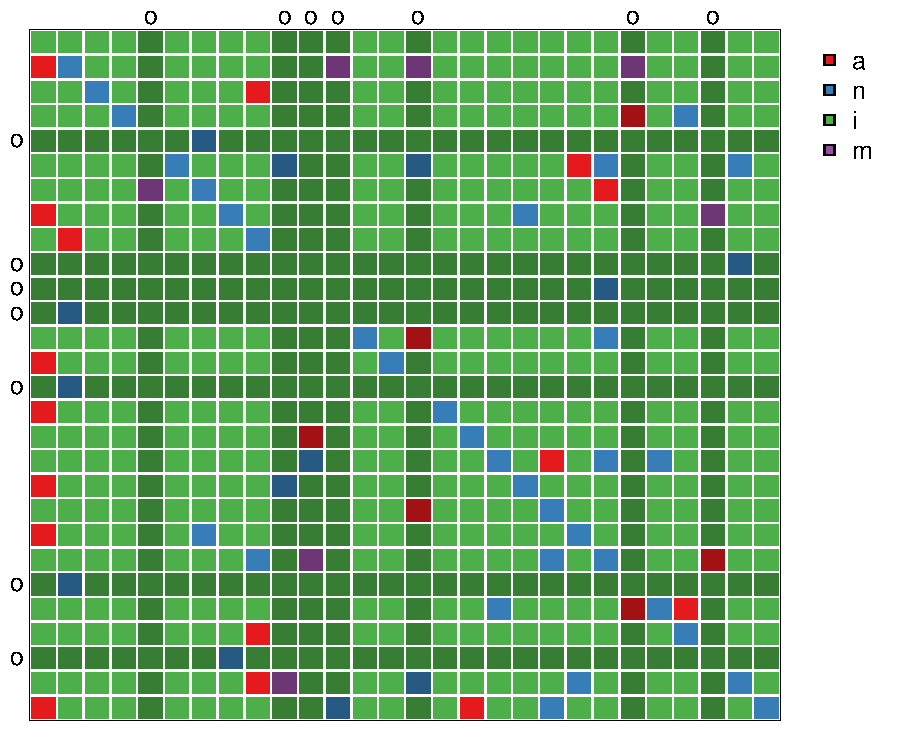
\includegraphics[width=0.45\textwidth]{matrix.pdf}
\caption{
An example of the source pool interaction matrix where $\mathcal{S} = 50$. Species and objects are aligned across the rows and columns; objects are shaded and labeled by `o' to distinguish them from species. The interaction recorded in row $i$ and column $j$ describes the directed interaction from species/object $i$ to species/object $j$. The first row/column represents the basal resource; species that assimilate the primary resource are capable of primary production. Species interact with other species and/or objects; objects only interact with their engineers by `needing' them; objects do not interact with other objects.
}
\label{fig:matrix}
\end{figure}


%
% %Interaction types
%
% The ENIgMa model consists of four directed interactions:
% $\rr{e}$: eat, which specifies a dependency involving the exchange of biomass,
% $\rr{n}$: need, which specifies a dependency that does not involve biomass flow (e.g. a reproductive service),
% $\rr{i}$: ignore, the null interaction, and
% $\rr{m}$: make, which connects a species to an object that it engineers.
% `Objects' are interactive components that can be made by $\geq 1$ species, and eaten, needed, or ignored by the others.
% The four directed interaction types describe specific dependencies that one species/object has on another, however it is the coupling of two opposing directed interactions that describe familiar ecological relationships (Table 1).
%
% The $\rr{e} \leftrightarrow \rr{i}$ interaction describes a typical predator-prey relationship, where species 1 eats species 2, whereas aside from serving as a resource, species 2 does not interact with (ignores) species 1.
% Of course, a prey's abundance does not \emph{ignore} the effects of predation, however our framework operates at the scale of presence/absence rather than abundance, and we assume that if both species co-occur, they have positive population densities, such that the prey's state (presence/absence) ignores the predator.
% A second type of trophic interaction is described by $\rr{e} \leftrightarrow \rr{e}$, where consumption is symmetric, which could be do to changing roles over an individual's life-history.
% The $\rr{e} \leftrightarrow \rr{n}$ and $\rr{n} \leftrightarrow \rr{n}$ interactions describe service-resource and service-service mutualisms, respectively.
% In the case of the former, one species interacts by way of a trophic interaction, whereas the other is provided a non-trophic need, such is the case in a plant-pollinator relationship.
% Unique to models of ecological networks, the $\rr{m} \leftrightarrow \rr{n}$ interaction describes ecosystem engineering, where a species makes an object, whereas the presence of the object `needs' the presence of the species that makes it.
% Objects can be utilized by other species in the community, providing an indirect dependency that could be facilitated by multiple species (many engineers make the same object) and/or used by multiple species (many species eat or need the same object).
% As we will describe below, engineers can modify the niche space available to the community on timescales that last longer than the species themselves, which is an oft-assumed characteristic of engineering.
%
% We explore the assembly of a novel community that emerges from a species source pool, which is represented by a source pool interaction matrix where all eat, need, ignore, and make interactions are established between all species and objects.
% As such, a set of interactions for a particular species defines how it interacts with any other \emph{a priori}, thereby establishing its potential interaction niche space.
% The source pool is used to seed a novel community, which arises as the result of colonization and extinction rules, the details of which we describe below.
%

\bibliography{aabib}

\end{document}
